
\usetikzlibrary{arrows.meta}


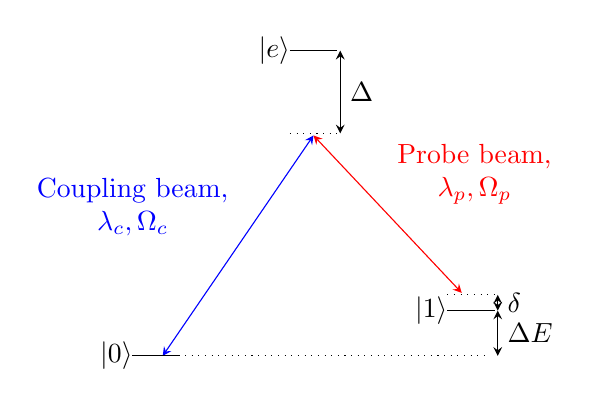
\begin{tikzpicture}
  % Lower energy levels
  \node(0) at (0,0) {};
  \node[label=left:$\vert 0 \rangle$] (0_label) at (-0.05,0.125) {};
  \node[label=left:$\vert 1 \rangle$] (1) at (4-0.05,0.7) {};
  \node[label=left:$\vert e \rangle$]  (e) at (2-0.05,4) {};
  \node (Delta) at (2,2.8) {};
  \node (delta) at (4,0.8) {};

  % Transitions
  \draw[<->,>=stealth,blue] (0) -- node[above left, align=center] {Coupling beam, \\ $\lambda_c, \Omega_c$} (Delta.north);
  \draw[<->,>=stealth,red] (delta) -- node[above right, align=center] {Probe beam, \\ $\lambda_p, \Omega_p$} (Delta.north);

  % Horizontal lines under node names
  \draw (-0.3,0.125) -- (0.3,0.125); % <-- Modify this
  \draw (3.7,0.7) -- (4.3,0.7); % <-- And this
  \draw (1.7,4) -- (2.3,4); % <-- And this
  \draw[dotted] (1.7,2.95) -- (2.3,2.95);
  \draw[dotted] (3.7,0.9) -- (4.3,0.9);
  \draw[dotted] (0.2,0.125) -- (4.2,0.125);

  \draw[<->,>=stealth] (2.34,2.95) -- node[right] {$\Delta$} (2.34, 4);
  
  \draw[<->,>=stealth, arrows={<->[scale=0.1]}] (4.34,0.7) -- node[right] {$\delta$} (4.34, 0.9);
  \draw[<->,>=stealth, arrows={<->[scale=0.1]}] (4.34,0.7) -- node[right] {$\Delta E$} (4.34,0.125);
\end{tikzpicture}
